% ISE conference template using Gemini project
% https://github.com/anishathalye/gemini

\documentclass[final,20pt]{beamer}

% ====================
% Packages
% ====================

\usepackage[T1]{fontenc}
\usepackage{lmodern}
\usepackage[size=custom,width=76.2,height=120,scale=1.2]{beamerposter}
\setlength{\paperwidth}{30in}
\setlength{\paperheight}{40in}
\usetheme{gemini}
\usecolortheme{gemini}
\usecolortheme{beaver}

\usepackage{amsmath,amsthm}
\usepackage{graphicx}
\usepackage{booktabs}
\usepackage{tikz}
\usepackage{pgfplots}
\pgfplotsset{compat=1.18}
\usepackage{anyfontsize}
\usepackage{comment}


% ====================
% Lengths
% ====================

% If you have N columns, choose \sepwidth and \colwidth such that
% (N+1)*\sepwidth + N*\colwidth = \paperwidth
\newlength{\sepwidth}
\newlength{\colwidth}
\setlength{\sepwidth}{0.025\paperwidth}
\setlength{\colwidth}{0.3\paperwidth}

\newcommand{\separatorcolumn}{\begin{column}{\sepwidth}\end{column}}

% ====================
% Title
% ====================

\title{Nash Equilibrium of\texorpdfstring{\\}{ }Hand Cricket}

\author{Aniket Murhekar \inst{1} \and Eklavya Sharma \inst{2}}

\institute[shortinst]{\inst{1} aniket2@illinois.edu \samelineand \inst{2} eklavya2@illinois.edu}

% ====================
% Footer (optional)
% ====================

\footercontent{\Large ISE Student Conference 2024\vspace{15px}}
% (can be left out to remove footer)

% ====================
% Logo (optional)
% ====================

% use this to include logos on the left and/or right side of the header:
\logoright{
\includegraphics[scale=1.8]{img/ISEmod.png}}
\logoleft{
\includegraphics[scale=1.3]{img/logo3.pdf}}

% ====================
% Macros
% ====================

\newcommand*{\defeq}{:=}
\DeclareMathOperator{\graph}{graph}

% ====================
% Body
% ====================

\begin{document}

\begin{frame}[t]
\begin{columns}[t]
\separatorcolumn

\begin{column}{\colwidth}

\begin{block}{Hand Cricket and RUC Games}

\emph{Hand cricket} is a two-player game played with hand gestures (like rock-paper-scissors).
It is popular among children in India.

We generalize hand cricket to \emph{Repeat-Until-Collision (RUC) games}.
Parametrized by matrices $A, B \in \mathbb{R}_{\ge 0}^{n \times n}$.
Rules:
\begin{enumerate}
\item There are two players: max player (aka batter) and min player (aka bowler).
\item There are multiple rounds. In each round, both players simultaneously
    pick a number from $\{1, 2, \ldots, n\}$.
\item If max player picks $i$ and min player picks $j$,
    max player scores $A[i, j]$, min player incurs a cost of $B[i, j]$.
\item If $i = j$, the game ends. Else, proceed to next round.
\item Max player wants to maximize her (expected) total score.
    Min player wants to minimize her (expected) total cost.
\end{enumerate}

Hand cricket: $A[i, j] = B[i, j] = i$.

\begin{figure}[htb]
\centering
\raisebox{-0.5\height}{
\includegraphics[scale=0.45]{img/hand5.png}}%
\hfill
\raisebox{-0.5\height}{
\includegraphics[scale=0.5]{img/hand2.png}}%
\caption{Single round of hand cricket, where max player (left) played 5 and min player (right) played 2.
Max player earned 5 points. Min player incurred a cost of 5 points.
$5 \neq 2$, so game doesn't end.}
\end{figure}

Max-player can score more per round by playing high-scoring actions, but then the game can end sooner.
Playing \emph{optimally} requires carefully balancing this tradeoff.

%Lorem ipsum dolor sit amet, consectetur adipiscing elit. Morbi ultricies
%eget libero ac ullamcorper. Integer et euismod ante. Aenean vestibulum
%lobortis augue, ut lobortis turpis rhoncus sed.

\end{block}

\end{column}

\separatorcolumn

\begin{column}{\colwidth}

\begin{block}{Pursuit-Evasion Games}

\begin{figure}[htb]
\centering
\raisebox{-0.5\height}{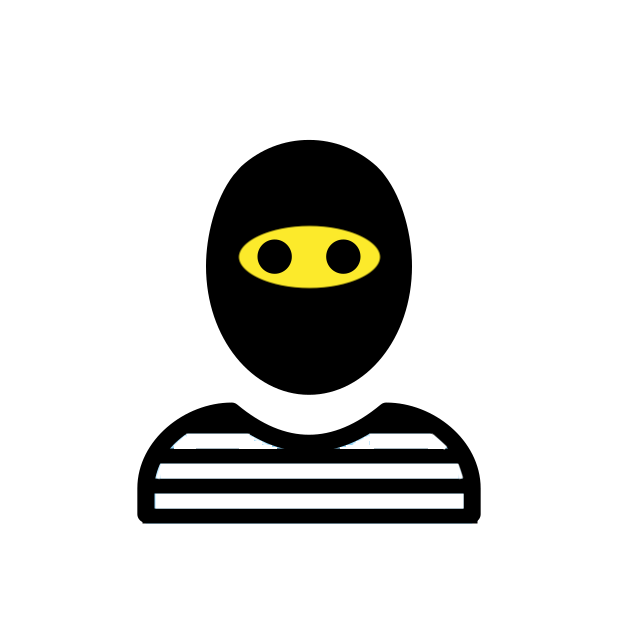
\includegraphics[scale=0.5]{img/burglar.png}}%
\hfill
\raisebox{-0.5\height}{
\includegraphics[scale=0.5]{img/police.png}}%
\end{figure}

There are $n$ locations. Each day, a drug dealer picks a location to sell drugs,
and law enforcement picks a location for a random check.
If the locations match, the dealer is caught and the game ends.
This is another example of an RUC game.

\end{block}

\begin{block}{Nash Equilibria}

A pair $(x, y)$ of strategies if called a \emph{Nash Equilibrium} (NE) if both of these hold:
\begin{enumerate}
\item If min player plays $y$, then playing $x$ maximizes max player's score.
\item If max player plays $x$, then playing $y$ minimizes min player's cost.
\end{enumerate}

\end{block}

\begin{alertblock}{Our Results}

Let $\Delta_n \defeq \{x \in \mathbb{R}_{\ge 0}^n: \sum_{i=1}^n x_i = 1\}$.

\emph{Stationary strategy} $x \in \Delta_n$:
pick each action $i$ with probability $x_i$ independently in each round.

A \emph{stationary RUC (SRUC) game} is one where both players are
forced to play only stationary strategies.

\textbf{Theorem 1.}
Let $A$ and $B$ be irreducible matrices.
\begin{enumerate}
\item $\exists x, y \in \Delta_n$ such that
    $(x, y)$ is an NE for both the SRUC game and the RUC game.
\item NE is unique for SRUC game iff $\graph(A) \subseteq \graph(B)$.
\item NE is almost-unique for RUC game if $A = B$.
\end{enumerate}

\end{alertblock}

\end{column}

\separatorcolumn

\begin{column}{\colwidth}

\begin{block}{Proof Sketch}

\heading{SRUC Games}

\textbf{Theorem 2.}
If max player plays $x \in \Delta_n$ and min player plays $y \in \Delta_n$,
then max player's expected total score is $x^TAy/x^Ty$
and min player's expected total cost is $x^TBy/x^Ty$.

\begin{itemize}
\item If $y$ is $A$'s eigenvector, max player's score is independent of $x$.
\item If $x$ is $B^T$'s eigenvector, min player's cost is independent of $y$.
\end{itemize}

If such eigenvectors exist, they would give us NE.
But do they exist? Yes!

\textbf{Perron-Frobenius Theorem.}
Let $A \in \mathbb{R}_{\ge 0}^{n \times n}$ be irreducible. Then
\begin{enumerate}
\item \emph{(Perron root)}
    $\exists$ eigenvalue $\rho \in \mathbb{R}_{\ge 0}$ that is largest in absolute value
    among all (complex) eigenvalues.
\item \emph{(Perron vectors)}
    $\exists$ unique vectors $u$ and $v$ s.t. $A^Tu = \rho u$, $Av = \rho v$,
    and $\sum_{i=1}^n u_i = \sum_{i=1}^n v_i = 1$.
\item $u_i > 0$ and $v_i > 0$ for all $i$.
\end{enumerate}

\textbf{Example:}
If $A = \begin{bmatrix}0 & s_1 \\ s_2 & 0\end{bmatrix}$, then
$\rho = \sqrt{s_1s_2}$, $u = (1 - \alpha, \alpha)$, and $v = (\alpha, 1 - \alpha)$,
where $\alpha = \displaystyle\frac{\sqrt{s_1}}{\sqrt{s_1} + \sqrt{s_2}}$.

\heading{RUC Games}

RUC games have a recursive structure:
after the first round, if the game doesn't end,
the remaining game is identical to the original.
\end{block}

\begin{block}{Paper}

Published in conference FSTTCS 2023.
\href{https://doi.org/10.4230/LIPIcs.FSTTCS.2023.18}{\texttt{doi:10.4230/LIPIcs.FSTTCS.2023.18}}

\begin{figure}
\centering

\includegraphics[scale=1.0]{img/hc-doi.png}
\end{figure}

\end{block}

\end{column}

\separatorcolumn
\end{columns}

\end{frame}

\end{document}
